% This is samplepaper.tex, a sample chapter demonstrating the
% LLNCS macro package for Springer Computer Science proceedings;
% Version 2.21 of 2022/01/12
%
\documentclass[runningheads]{llncs}
%
\usepackage[T1]{fontenc}
% T1 fonts will be used to generate the final print and online PDFs,
% so please use T1 fonts in your manuscript whenever possible.
% Other font encondings may result in incorrect characters.
%
\usepackage{graphicx}
\usepackage{amsmath}
\usepackage{algorithmicx}
\usepackage{algorithm}
\usepackage[noend]{algpseudocode}

\makeatletter
\def\BState{\State\hskip-\ALG@thistlm}
\makeatother
% Used for displaying a sample figure. If possible, figure files should
% be included in EPS format.
%
% If you use the hyperref package, please uncomment the following two lines
% to display URLs in blue roman font according to Springer's eBook style:
%\usepackage{color}
%\renewcommand\UrlFont{\color{blue}\rmfamily}
%
\begin{document}
%
\title{Linear-Space Data Structure for Parametrized Range Mode Query in Arrays\thanks{Supported by Alexandru Ioan Cuza Universy of Iași.}}
%
%\titlerunning{Abbreviated paper title}
% If the paper title is too long for the running head, you can set
% an abbreviated paper title here
%
\author{Ovidiu Rața\inst{1}, Paul Flavian Diac\inst{1}}
%
% First names are abbreviated in the running head.
% If there are more than two authors, 'et al.' is used.
%
\institute{Alexandru Ioan Cuza Universy of Iași,\\ Faculty of Computer Science, Iași, Romania}
%
\maketitle              % typeset the header of the contribution
%
\begin{abstract}
We present a data structure for the range mode query problem, studied by Chan et al \cite{chan2014linear}, He,Liu.\cite{he_et_al:LIPIcs.SEA.2023.19} and Xu, Williams et al\cite{gu2021faster}, which requires $O(n)$ space,
and answers queries on an interval $[i, j]$ in parametrized $O(\sqrt{j-i+1})$ time. The standard RAM model is assumed, with word size $w = \Theta ( \log n )$.\\

Additionally, we present a linear-space data structure, that requires \\ 
$O(\min( \sqrt{j-i+1}, \sqrt{j/w} ) )$ parametrized time per query, 
and supports element insertion at the end of the array $A[1:n]$ in amortyzed $O( w + \sqrt{n \cdot w} )$ time, by improving over the method proposed by Chan et al\cite{chan2014linear}, using compact rank/select data structures 
that support appending an element at the end of the binary array in amortyzed $O(1)$ time.


\keywords{ Data structure  \and Parametrized algorithms \and Range queries \and Mode.}
\end{abstract}
%
%
%
\section{Introduction}

\section{Finding a Range Mode}
Our data structure is constructed by extending the ideas of Chan et al\cite{chan2014linear}.

\subsubsection{Data Structure precomputation.} Let $D$ denote the set of elements of the array $A$, and assume some arbitrary ordering on the elements. 
We will maintain $D$, as a red-black tree.
We denote the number of distinct elements of $A$ as $\Delta$. First, we apply rank-space reduction, and 
construct the array $B$, such that, for each $i$, $B[i]$ stores the rank of $A[i]$ in $D$. Thus, $B[i]\in \{1,\dots, \Delta\}$.
Let $C$ be an array of size $\Delta$, that provides a direct mapping from $\{1,\dots,\Delta\}$ to $D$. Set $D$ and arrays $B$ and $C$
can be computed inf $O(n \log\Delta )$ time. Further, we will focus on finding a range mode $x$, over array $B$, which will be transformed into the 
respective range mode over array $A$, using array $C$, that is, $y=C[x]$.
For each $a\in \{1,\dots \Delta\}$, let $Q_a = \{ b\ |\ B[b]=a  \} $. We will represent the sets $Q_a$ as ordered arrays. Also, we define the array $Q^{-1}$, of size $n$, s.t. $\forall i \in \{1,\dots ,n\}, Q^{-1}_i=k, Q_{B_i}(k)=i$.

%We also declare array $E$ of size $\delta$, which initially has all entries set to $0$, and which will be used to store the 
%frequency values calculated for individual elements of array $B$, during queries. 
%After each query, the accessed entries of array $E$ will also be set back to $0$.\\

%The main idea behind the construction of the data structure, is to separate it into $\lfloor log  n \rfloor + 1 $ levels, numbered $0$ through 
%$\lfloor log n \rfloor $. Level $l$, will correspond to 

\subsubsection{Additional Definitions.}
Let $\phi(i,j)$ be the function that returns the frequency of the most frequent element in the range $B[i:j]$.

Let $\textbf{freq}_x(i,j)$, be the frequency of element $x$ of array $B$, inside the interval $[i,j]$.


Further, we will show how to build a data structure, that supports parametrized range mode query in time $O(\sqrt{j-i+1})$ for a query interval
$[i,j]$.


\begin{lemma}
    Given an array $A[1:n]$, there exists a data structure, requiring arrays $B$, $C$, $Q$, $Q^{-1}$, the set $D$, and $ O(n/w) $ additional words of RAM, that for some fixed integer 
    $L \in \{ 0 , \cdots , \lceil  \log n \rceil \}$, for intervals $[i,j]$ s.t. $ 2^{L-1} < j-i+1 \leq 2^L$
    supports queries of the following form, in $O(\sqrt{2^L})$ time: 

    For the interval $[i,j]$, determine an element $x$, s.t. $\textbf{freq}_x(i,j) \geq \min(\phi(i,j), \sqrt{2^L})$

    % for the most frequent element, in $O(\sqrt{2^L} )$ time, over intervals , for elements, whose frequency in the interval $[i,j]$ is $\leq \sqrt{2^L}$
\end{lemma}
\begin{proof}
    First, we fix an integer $L \in \{ 0 , \cdots , \lceil  \log n \rceil \}$.
    Then, we separate the array $A[1:n]$ into adjacent blocks, of length $b_L = \sqrt{2^L}$. The block $i\in \{1,\dots, \lfloor \frac{n}{b_L} \rfloor\}$ 
    encompasses the interval $[(i-1) \cdot b_L +1, \min(i\cdot b_L , n)]$.

    \begin{figure}[H]
        \centering
        \hspace*{-0.5cm}      
        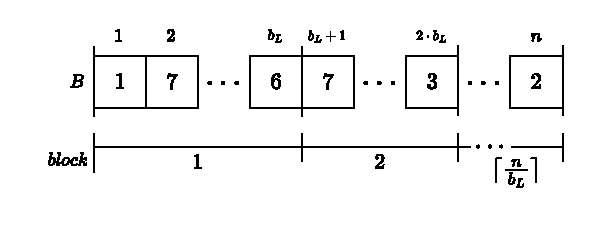
\includegraphics[scale=0.8]{figures/example_figure1.pdf}
        \caption{ Example of separating an array $B$ into $\lceil \frac{n}{b_{L}} \rceil$ adjacent blocks of length $b_{L}=\sqrt{2^L}$. }
        \label{fig:fig1}
    \end{figure}
    
    Let $s_i^L$, be a binary string, similar to the string defined in the data structure proposed by Chan et al.\cite{chan2014linear}:
    
    \begin{definition}
        For integer $L \in \{ 0 , \cdots , \lceil  \log n \rceil \}$, and block $i$ of size $\sqrt{2^L}$, let $s_i^L$ be a binary string, obeying the following properties:
        
        \begin{property}
            Consider the interval of blocks, from block $i$ to block $j=\min( \lfloor \frac{n}{b_L} \rfloor, i+\sqrt{2^L}-1 )$.
            There will be $j-i+1=O(\sqrt{2^L})$ bits with value $1$ in $s_i^L$, the $k$-th set bit corresponding to the right border of the interval $k$.        
        \end{property}

        \begin{property}
            For any integer $k\in [i,j]$, consider the interval of blocks $[i,k]$.

            For the interval of blocks $[i,k]$, consider the endpoints of array $A$ which correspond to the left endpoint of the block $i$, and the right endpoint of the block $k$ 
            to be $i'=(i-1)\cdot b_L+1, k'=k\cdot b_L$.

            In the string $s_i^L$, there are exactly $\min(\sqrt{2^L}, \phi(i',k') )$ bits with value $0$ to the left of the $k$-th set bit. 
        
        \end{property}

    \end{definition}
    
    Note that the length of the binary string $s_i^L$ is at most $ 2\cdot \sqrt{2^L} = O(\sqrt{2^L})$.
    
    Every string $s_i^L$, can be represented with a succint or compact data structure that supports rank-select operations, in $O(\sqrt{2^L}/w)$ RAM words.
    
    There are $\lfloor \frac{n}{2^L} \rfloor$ blocks of length exactly $b_L$, thus, the space necessary for maintaining the strings $s_i^L$ is:
    \[
        \lfloor \frac{n}{2^L} \rfloor \cdot O(\sqrt{2^L}/w) = O(n/w) \text{ words of RAM. }
    \]


    \begin{figure}[H]
        \centering
        \hspace*{-1.2cm}      
        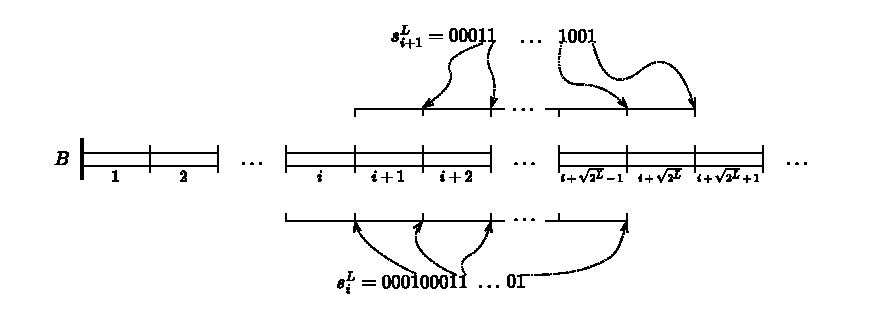
\includegraphics[scale=0.8]{figures/example_figure2.pdf}
        \caption{ Example of strings $s_{i}^{L}$ and $s_{i+1}^{L}$ over an array $B$, separated into blocks of size $b_L$. 
        Each bit with value $1$ in the strings $s_{i}^L$ and $s_{i+1}^L$ represents the right border of some block. }
        \label{fig:fig2}
    \end{figure}


    \subsubsection{Query Algorithm.} The query alorithm is similar to that of the data structure proposed by Chan et al.\cite{chan2014linear}:

    \begin{enumerate}
        \item[] Given the interval $[i,j]$:
        \item If $j-i+1\leq 2\cdot \sqrt{2^L}$, then just iterate through the elements of $[i,j]$ in $O(\sqrt{2^L})$ time, or determine the blocks that are entirely contained inside of $[i,j]$.
         Let the block and the last blocks be $\beta_1$ and $\beta_2$ respectively.  
        \item There will be at most $\sqrt{2^L}$ blocks from block $\beta_1$ to block $\beta_2$.
        
         Let $[i', j']$ be the interval of $A$, which corresponds to blocks $\beta_1$ through $\beta_2$.
         We will use the string $s^L_{\beta_1}$ to get the frequency $f$, of an element from $[i',j']$ s.t. $f \geq \min( \phi(i',j'),\sqrt{2^L} )$.
         This can be done by select operations over $s^L_{\beta_1}$, more precisely, we will determine $p=\textbf{select}_1(s^L_{\beta_1}, \beta_2-\beta_1+1 )$, 
         which is the position in the string $s^L_{\beta_1}$, corresponding to the right endpoint of the block $\beta_2$, with respect to block $\beta_1$. 
        The value $f$, corresponding to the number of bits with value $0$ in the interval $[1 , p_2]$ of the string $s^L_{\beta_1}$, can be calculated as follows:
         \[
            f = (p)-(\beta_2-\beta_1+1)
         \]
        We can further use binary search, to get the number $\beta_f$ and the position $p_f$ in string $s^L_{\beta_1}$ of the first block, such that there are exactly $f$ bits with value $0$ in the interval 
        $[1,  p_f]$ of the string $s^L_{\beta_1}$. 
        Further, we can iterate through each position $k$, of the block $\beta_f$, and use arrays $Q_{B_k}$ in order to determine an element $ x $ with frequency at least $f$. (Chan et al.\cite{chan2014linear}) 

        This procedure will take $O(\sqrt{2^L})$ time, as the most time consuming step is the iteration through elements of $\beta_f$.
         
        We must also note, that this step will yield exactly the answer for the query $(i',j')$.

         \item Further, we can iterate through each position $k\in ([i,j]\setminus [i', j'])$, 
         and increase $f$ every time we can if it is $<\sqrt{2^L}$, by checking whether $Q_{B_k}(Q^{-1}_k \pm (f+1) ) \in [i,j]$. This will clearly take $O(\sqrt{2^L} )$ time, as there will be $O(\sqrt{2^L})$ elements in the prefix and suffix of $[i,j]$, and we will 
         increase $f$ at most $O(\sqrt{2^L})$. 

         This step clearly determines the answer for the query $[i,j]$, as it uses the value $f$ characterising the answer for the query $(i',j')$, and uses the prefix and suffix of $[i,j]$, in order to adapt $f$ 
         to the answer for the query $(i,j)$. These steps are the same as in the data structure proposed by Chan et al.\cite{chan2014linear}, and proofs for their correctness are also provided in their work. 

        \end{enumerate}
        
        Finally, the required element $x$ of the range $B[i:j]$, can be transformed to the corresponding element of $A$, which is $C_{ x }$. 
        Thus, the answer to the query $(i,j)$ given above, is calculated in $O(\sqrt{2^L})$ time.$\qed$ 



\begin{algorithm}[H]
    \caption{Lemma 1 Query Algorithm}\label{lemma1Query}
    \begin{algorithmic}[1]
    \Function{Query}{}
    
    \Comment{Step 1:}

    \If {$j-i+1\leq 2\cdot \sqrt{2^L}$}
    \State \#Iterate through each element of [i,j] and return the answer.
    
    \EndIf
    \State $\beta_1 \gets \lfloor \frac{i-1}{ \sqrt{2^L} } \rfloor +1, \beta_2 \gets \lfloor \frac{j}{\sqrt{2^L}} \rfloor$
    \State $i' \gets (\beta_1-1) \cdot \sqrt{2^L} + 1 , j' \gets \beta_2 \cdot \sqrt{2^L} $
    
    \Comment{Step 2:}
    \State $p \gets \textbf{select}_1(s^L_{\beta_1}, \beta_2-\beta_1+1 ), f \gets (p)-(\beta_2-\beta_1+1) $
    
    \State \# Find $\beta_f$ and $p_f$, and iterate through the block $\beta_f$, and get the candidate element $x$.

    \Comment{Step 3:}

    \For{$k \in [i,i'-1]$}
        \While{$Q_{B_{k}}( Q^{-1}(k)+f+1 )\leq j$ and $f<\sqrt{2^L}$}
            \State $f\gets f+1$
            \State $x\gets B_k$
        \EndWhile
    \EndFor

    \For{$k \in [j'+1,j]$}
        \While{$Q_{B_{k}}( Q^{-1}(k)-f-1 )\geq i$ and $f<\sqrt{2^L}$}
            \State $f\gets f+1$
            \State $x\gets B_k$
        \EndWhile
    \EndFor

    \Return $(C(x),f)$

    \EndFunction
    \end{algorithmic}
\end{algorithm}


\end{proof}


Further, for any integer $L \in \{ 0 , \cdots , \lceil  \log n \rceil \}$ we will define $b_L'=2^L$, as the size of the big blocks, and will separate the array $B[1:n]$ into adjacent blocks of size $b_L'$.
If we cannot exactly divide the array $B[1:n]$ into blocks of size $b_L'$, then the last elements of array $B[1:n]$ will just be included into a last block, of size $<b_L'$.

For every block $i\in\{ 1,\dots,\lceil \frac{n}{b_L'} \rceil \}$ of size $b_L'$, we denote by $F_i^L$, the set of elements in the range $B[(i-1) \cdot b'_L +1: \min((i+1)\cdot b_L' , n)]$, that have frequency $>\sqrt{2^L}$. 
Note that the interval $[(i-1) \cdot b'_L +1: \min((i+1)\cdot b_L' , n)]$ contains $2$ big blocks, if its size is not limited by $n$.  

If we maintain the sets $F_i^L$ as ordered arrays, then the amount of space required for storing $F_i^L$ will be:
\[
    \sum_{L=0}^{\lceil \log n \rceil} \sum_{i=1}^{\lceil \frac{n}{b_L'}\rceil } |F_i^L| \leq \sum_{L=0}^{\lceil \log n \rceil} \sum_{i=1}^{\lceil 2 \cdot \frac{n}{b_L'}\rceil } 2\cdot \sqrt{2^L} 
\]
\[
    = O(  \sum_{L=0}^{\inf} \sum_{i=1}^{ \lfloor \frac{n}{2^L} \rfloor } \sqrt{2^L} ) = O( \sum_{L=0}^{\inf} \lfloor \frac{n}{2^L} \rfloor \cdot \sqrt{2^L} )
\]

\[
    = O( \sum_{L=0}^{\inf} \frac{n}{\sqrt{2^L}} ) = O( \sum_{L=0}^{\inf} \frac{n}{\sqrt{2^L}}  ) = O( n \cdot \sum_{L=0}^{\inf} \frac{1}{\sqrt{2^L}}  )
\]
\[
    = O( n \cdot \frac{ \sqrt{2} }{ \sqrt{2} - 1 }  ) = O(n)
\]


Thus, storing the sets $F_i^L$ is $O(n)$ words of RAM, as storing each element of $F_i^L$ requires $1$ word of RAM.

\begin{lemma}
    Given an array $A[1:n]$, there exists a data structure, requiring arrays $B$, $C$, $Q$, $Q^{-1}$, $F_i^L$, the set $D$, and $ O(n/w) $ additional words of RAM, that for some fixed integer 
    $L \in \{ 0 , \cdots , \lceil  \log n \rceil \}$, for intervals $[i,j]$ s.t. $ 2^{L-1} \leq j-i+1 < 2^{L}$
    and supports queries of the following form, in $O(\sqrt{2^L})$ time:

        For the range $A[i:j]$, determine an element of frequency $\phi(i,j)$, if $\phi(i,j)>\sqrt{2^L}$, or $-1$ if no such element exists. 
\end{lemma}
\begin{proof}
    First, we fix an integer $L \in \{ 0 , \cdots , \lceil  \log n \rceil \}$.
    Then, we separate the array $A[1:n]$ into adjacent blocks, of length $b_L' = 2^L$. The block $i\in \{1,\dots, \lceil \frac{n}{b'_L} \rceil\}$ 
    encompasses the interval $[(i-1) \cdot b'_L +1, \min(i\cdot b_L' , n)]$.
    
    For each element $x$ in $F_i^L$, we define the binary string $Y_{i,x}^L$, the following way:
    \begin{definition}
        For integer $l \in \{ 0 , \cdots , \lceil \log n \rceil \}$, for each block $i$ of size $2^L$, for each element $x \in F_i^L$, let $Y_{i,x}^L$ be a binary string, obeying the following properties:
       \begin{property}
        The string $Y_{i,x}^L$ will have at most $2\cdot \sqrt{2^L}$ bits set to value $1$. Each of these bits, will correspond to the right endpoint of a small block of size $b_L=\sqrt{2^L}$, declared in \textbf{lemma 1},
         that lies inside the big block $i$, of size $b_L'$, or in the big block $i+1$.
       \end{property}

       \begin{property}
            For every $k$, from $1$ to  $2\cdot \sqrt{2^L}$, let $k'=\min(k'\cdot b_L+i', n)$ be the right endpoint of the $k$-th small block, counting from the first small block inside of the big block $i$, or just $n$, 
            if such a block does not exist. Note that the small block $k$ may lie inside the big block $i+1$.

            Inside the string $Y_{i,x}^L$, there will be exactly $\textbf{freq}_x(i',k')$ bits with value $0$ to the left of the $k$-th bit with value $1$.
        \end{property}

    \end{definition}


    \begin{figure}[H]
        \centering
        \hspace*{-1.2cm}      
        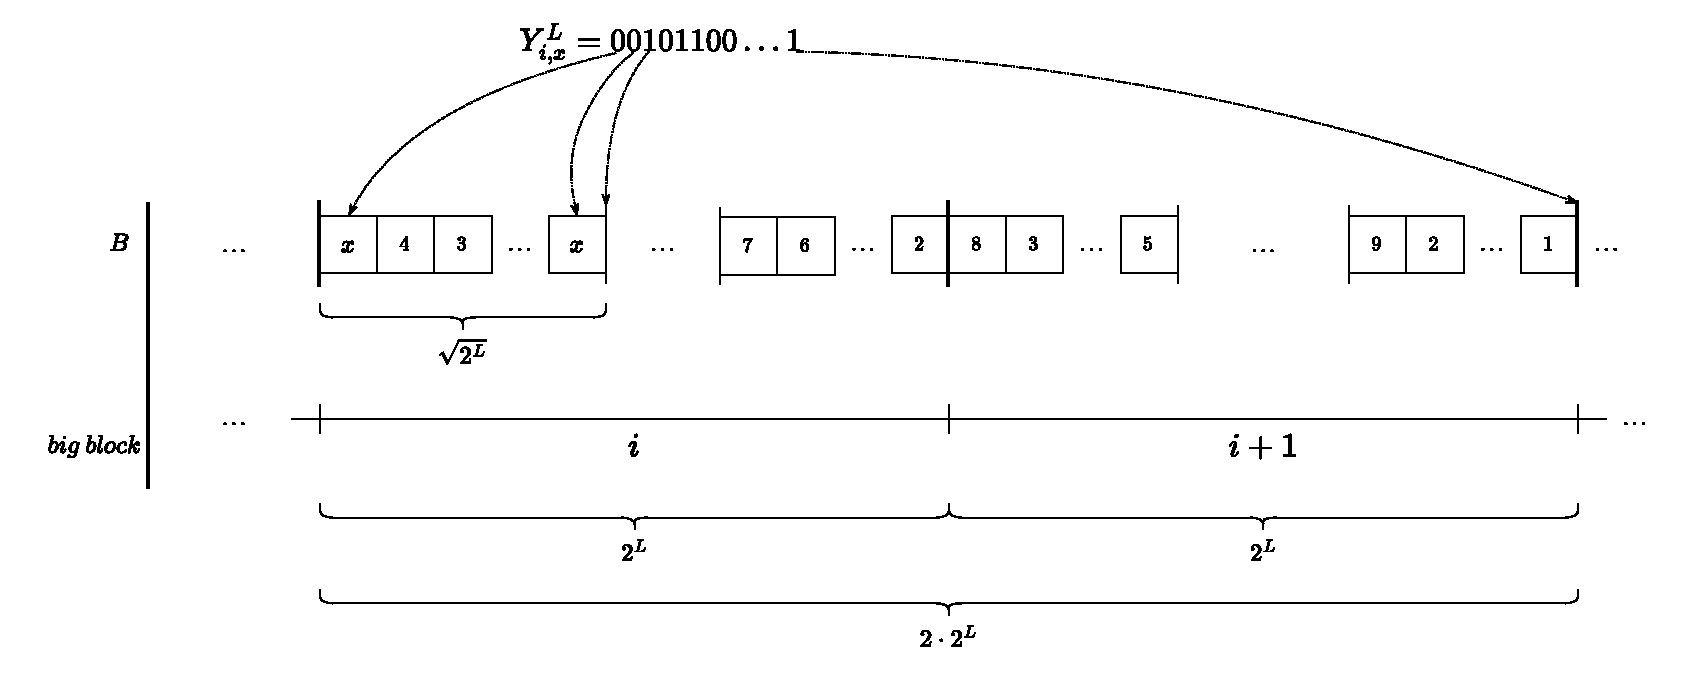
\includegraphics[scale=0.50]{figures/example_figure3.pdf}
        \caption{ Example of string $Y^{L}_{i,x}$ over an array $B$, for an element $x\in F_{i}^{L}$. The array $B$ separated into big blocks of size $b_L'$. The big block $i$ is in its turn separated into small blocks of size $b_L$.
            Each bit with value $1$ in string $Y^{L}_{i,x}$ corresponds to the right border of a small block of size $b_L$, and each bit with value $0$ corresponds to an encounter of the element $x$ in the array $B$.  
        }
        \label{fig:fig3}
    \end{figure}


    The string $Y_{i,x}^L$ will have exactly $\text{\textbf{size}}_0=\textbf{freq}_x(b_L'\cdot(i-1)+1, \min( b_L'\cdot (i+1), n) )$ bits with value $0$. 
    Note that $\text{\textbf{size}}_0>\sqrt{2^L}$.
    Also, there will be exactly $\text{\textbf{size}}_1=2\cdot \sqrt{2^L}$ bits with value $1$. Thus, the size of the string will be : $\text{\textbf{size}}_0+\text{\textbf{size}}_1 \leq 3 \cdot \text{\textbf{size}}_0$. 

    Thus, the total length of the strings $Y_{i,x}^L$, over the blocks $i\in \{1,\dots, \lceil \frac{n}{b'_L} \rceil\}$ will be:
    \[
        \sum_{i=1}^{\lceil \frac{n}{b_L'} \rceil } \sum_{x\in F_{i}^L } |Y_{i,x}^L| \leq \sum_{i=1}^{\lceil \frac{n}{b_L'} \rceil } \sum_{x\in F_{i}^L } 3 \cdot \text{\textbf{size}}_0
    \]
    \[
        = \sum_{i=1}^{\lceil \frac{n}{b_L'} \rceil } \sum_{x\in F_{i}^L } 3\cdot \textbf{freq}_x(b_L'\cdot(i-1)+1, \min( b_L'\cdot (i+1), n) )
    \]
    \[
        \leq \sum_{x\in F_{i}^L } 3\cdot 2 \cdot \textbf{freq}_x(1,n) \leq \sum_{x \in B[1:n]} 6 \cdot \textbf{freq}_x(1,n) = O(n)
    \]

    The total length of the strings $Y_{i,x}^L$ will be $O(n)$ bits, thus, for a fixed $L$, they will require $O(n/w)$ words of RAM to be stored, 
    and to support rank/select operations in $O(1)$.


    \subsubsection{Query Algorithm.} The query alorithm is as follows:

        \begin{enumerate}
            \item[] Given the interval $[i,j]$:
            
            \item If $j-i+1\leq 2\cdot \sqrt{2^L}$, then just iterate through the positions of $B[i,j]$ and determine the answer. 
            Otherwise, the interval $[i,j]$ will intersect, at most $2$ big blocks of size $b_L'$. Let these blocks be $\beta_1'$ and $\beta_2'$. 
            Let the interval of small blocks that are entirely covered by the interval $[i,j]$, be $[\beta_1, \beta_2]$. 
            These blocks can be determined rapidly, as $\beta_2=\lfloor j/b_L \rfloor$ and $\beta_1=\lfloor (i+b_L)/b_L \rfloor$, and similarly 
            for the big blocks $\beta_1'$ and $\beta_2'$.
            
            \item Further, we iterate through each element $x\in F_{\beta_1'}^L$, and determine :
            \[
                p_1^x = \textbf{select}_1( Y_{\beta_1',x}^L, \beta_1-(\beta_1'-1)\cdot \frac{b_L'}{b_L}-1 ) , 
                p_2^x = \textbf{select}_1( Y_{\beta_1',x}^L, \beta_2-(\beta_1'-1)\cdot \frac{b_L'}{b_L} ) 
            \]

            \[
                f_x=(p^x_2-p^x_1)-(\beta_2-\beta_1+1), f=\max_{x \in F_{\beta_1'}^L }( f_x )
            \]  
            
            \item Now, we iterate through the positions $k$ of the prefix and the suffix of the interval $[i,j]$, which are not contained in any of the 
            small blocks in the interval$[\beta_1, \beta_2]$, and check wether we can increase $f$ by $1$ or not, by verifying if $Q_{B_k}(Q^{-1}_k \pm (f+1) ) \in [i,j]$.
            
            \item Finally, if $f$ will achieve a value $>\sqrt{2^L}$, then return $f$, or $-1$ otherwise.

        \end{enumerate}
        
        \subsubsection{Analysis.}
        We can clearly see, that the runtime of the query algorithm will be $O(\sqrt{2^L})$, as the first step requires $O(1)$ time, 
        the second step requires $O(\sqrt{2^L})$ time, as at most $O(\sqrt{2^L})$ elements of the set $F_i^L$ will be verified and the \textbf{select} operations will take $O(1)$ time.
        The third step will also take $O(\sqrt{2^L})$ time, as there will be $O(\sqrt{2^L})$ elements of the prefix and the suffix which will have to be verified, and the value of $f$ 
        will be increases by $1$ at most $O(\sqrt{2^L})$ times. Note that the element $x$ with maximum frequency, can also be easily tracked during each step.   



        \begin{algorithm}[H]
            \caption{Lemma 2 Query Algorithm}\label{lemma2Query}
            \begin{algorithmic}[1]
            \Function{Query}{}
            
            \Comment{Step 1:}

            \If {$j-i+1\leq 2\cdot \sqrt{2^L}$}
            \State \#Iterate through each element of [i,j] and return the answer.
            
            \EndIf
            \State $b_L \gets \sqrt{2^L}, b_L' \gets 2^L$
            \State $\beta_1 \gets \lfloor \frac{i-1}{ b_L } \rfloor +1, \beta_2 \gets \lfloor \frac{j}{b_L} \rfloor$
            \State $\beta_1' \gets \lfloor \frac{i-1}{ b_L' } \rfloor +1, \beta_2' \gets \lfloor \frac{j}{b_L'} \rfloor$
            \State $i' \gets (\beta_1-1) \cdot \sqrt{2^L} + 1 , j' \gets \beta_2 \cdot \sqrt{2^L} $
            \State $f \gets -1 , m\gets -1$
            
            \Comment{Step 2:}
            \For{$x\in F^L_{\beta_1'}$}
                \State $p_1^x \gets \textbf{select}_1( Y_{\beta_1',x}^L, \beta_1-(\beta_1'-1)\cdot \frac{b_L'}{b_L}-1 )$
            
                \State $ p_2^x \gets \textbf{select}_1( Y_{\beta_1',x}^L, \beta_2-(\beta_1'-1)\cdot \frac{b_L'}{b_L} ) $
                
                \State $f_x\gets (p^x_2-p^x_1)-(\beta_2-\beta_1+1)$
                
                \If{$f_x>f$}
                \State $f\gets f_x$
                \State $m\gets x$
                \EndIf
                \EndFor
            
            \If{$m=-1$}
                \Return $(-1,-1)$
            \EndIf
            
            \Comment{Step 3:}

            \For{$k \in [i,i'-1]$}
                \While{$Q_{B_{k}}( Q^{-1}(k)+f+1 )\leq j$}
                    \State $f\gets f+1$
                    \State $m\gets B_k$
                \EndWhile
            \EndFor
            
            \For{$k \in [j'+1,j]$}
                \While{$Q_{B_{k}}( Q^{-1}(k)-f-1 )\geq i$}
                    \State $f\gets f+1$
                    \State $m\gets B_k$
                \EndWhile
            \EndFor
            
            \Comment{Step 4:}
            \If{$f\geq \sqrt{2^L}$}
            \Return $(C(m),f)$
            \Else{}
            \Return $(-1,-1)$
            \EndIf
        
            \EndFunction
            \end{algorithmic}
        \end{algorithm}

\end{proof}

Further, we will use the results from \textbf{lemma 1} and \textbf{lemma 2} to prove that a $O(\sqrt{j-i})$ runtime per query is possible, by using $O(n)$ space.

\begin{theorem} 
    Given an array $A[1:n]$, there exists a data structure, requiring arrays $B$, $C$, $Q$, $Q^{-1}$, the set $D$, and additional $O(n)$ words of RAM, that supports 
    range mode queries over an interval $[i,j]$ in time $O(\sqrt{j-i+1})$.
\end{theorem}
\begin{proof}
    Firstly, we will build the arrays $B$, $C$, $Q$, and $Q^{-1}$, which will take $O(n\log n)$ time and $O(n)$ space. 
    Also, for each $L\in \{0,\dots,\lceil \log n \rceil\}$, we will build $F^L_i$. It is easy to see, that this will take $O(n\log n)$ time, 
    and $O(n)$ space.

    Further, for each $L\in \{0,\dots,\lceil \log n \rceil\}$, we will build an instance of the data structure described in \textbf{lemma 1}, denoted by $DS_1^L$, and an instance of the data structure 
    described in \textbf{lemma 2}, denoted by $DS_2^L$. These instances will take $O(n)$ space, as the arrays $B$, $C$, $Q$, $Q^{-1}$ and $F^L_{i}$ will be shared among them, and the additional information 
    will take $O(\log n \cdot n/w) = O(n)$ space.

    \subsubsection{Query Algorithm.} The query algorithm is as follows:
        \begin{enumerate}
        
            \item[] Given the interval $[i,j]$:
            
            \item Determine the smallest $L$, s.t $2^{L-1}< (j-i+1) \leq 2^L$. Note that $2^L=O(j-i+1)$.
            
            \item We will determine $(f, x)=\max( DS_1^L.query(i,j) , DS_2^L.query(i,j) )$, where $DS_1^L.query(i,j)$, and $DS_2^L.query(i,j)$ denotes querying the instances $DS_1^L$ and $DS_2^L$, respectively, for the interval $[i,j]$.
             $(f,x)$ will be exactly the answer for the query $(i,j)$, as $f=\phi(i,j)$, and $x$ is an element of the array $A$, s.t. $\exists y, s.t.\text{ } (C_y=x) \land (\textbf{freq}_y(i,j)=f)$.

        
        \end{enumerate}

        \subsubsection{Analysis.}
        The algorithm will take $O(\sqrt{2^L})=O(\sqrt{j-i+1})$ time, as $2^L=O(j-i+1) \qed $. 


        

\end{proof}

\begin{lemma}
    Given an array $A[1:n]$, there exists a data structure requiring $O(n)$ words of RAM, that supports 
    range mode queries over an interval $[i,j]$ in $O( \sqrt{j/w}  )$ time.    
\end{lemma}
\begin{proof}
    Firstly, we build the arrays $B$, $C$, $Q$, $Q^{-1}$, and set $D$, as in the previous data structures.
    
    In their work, Chan et al.\cite{chan2014linear} have divided the array $A[1:n]$ into blocks of equal length, in order to prove their result.
    We will take a similar approach, one difference being that we will divide the array $A[1:n]$ into $O(\sqrt{w\cdot n})$ blocks of varying size.

    Firstly, we divide the array $A[1:n]$ into adjacent big blocks, block $i$ (counting from left to right) having size $i$. It is easy to see, that there will be at most $O(\sqrt{n})$ big blocks.
    Further, we will divide each big block $i$, into small blocks, of size $i/\sqrt{w}$.
    
    
    \begin{figure}[H]
        \centering
        \hspace*{-0.5cm}      
        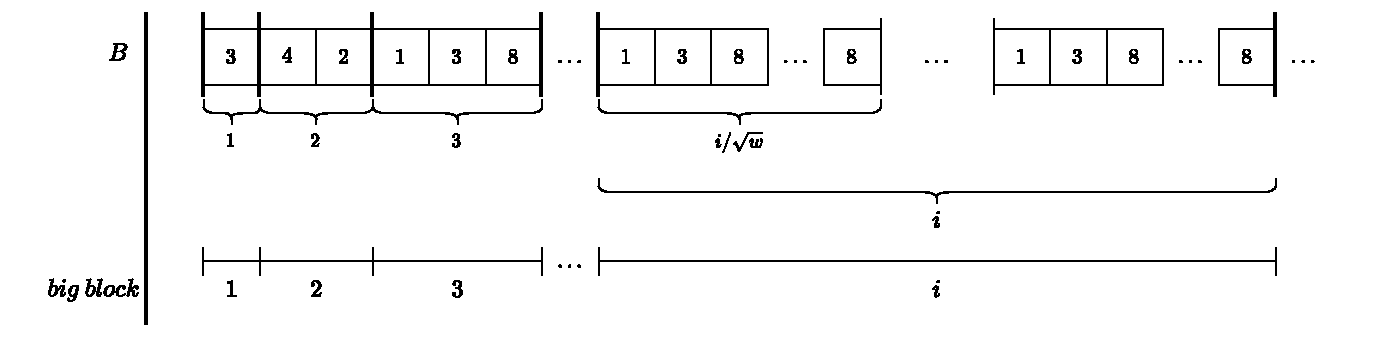
\includegraphics[scale=0.55]{figures/example_figure4.pdf}
        \caption{ Example of separating the array $B$ into big blocks. The big bocks $1,2,3$ have sizes $1,2,3$ respectively. The $i$-th big block has size $i$. 
        The $i$-th big block is in its turn divided into small blocks of size $i/\sqrt{w}$.}
        \label{fig:fig4}
    \end{figure}
    
    
    
    Let the number of small blocks be $b$. For each small block $\beta$ we will store the string $z_{\beta}$ and the set $H_{\beta}$, defined below:
    \begin{definition}
        For each small block $\beta\in\{1,\dots , b\}$, let $z_\beta$ be a binary string obeying the following properties:
        \begin{property}
            There are exactly $\beta$ bits with value $1$ in string $z_{\beta}$. The $k$-th bit with value $1$ counting from left to right will correspond to the left border of the $k$-th small block.    
        \end{property}

        \begin{property}
            For each bit $k$ with value $1$, let $l_k$ be the position of the left endpoint of the small block $k$ in array $B$, and let $r_{\beta}$ 
            be the position of the right endpoint of the small block $\beta$ in array $B$. 
            There will be exactly $\min(\phi(l_k,r_{\beta}) , b )$ bits with value $0$, to the right of the $k$-th bit with value $1$.
        \end{property}

    \end{definition}

    \begin{figure}[H]
        \centering
        \hspace*{-1cm}      
        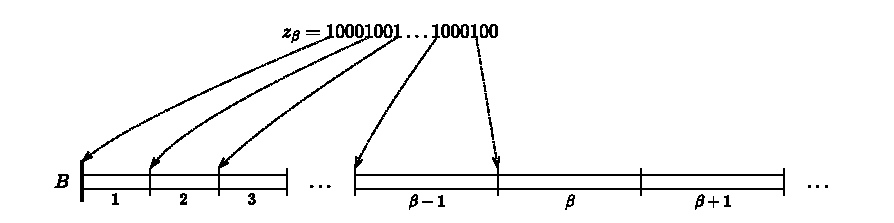
\includegraphics[scale=1]{figures/example_figure5.pdf}
        \caption{
            Example of a string $z_{\beta}$ over an array $B$. The array $B$ is illustrated as being separated into small blocks.
            The small blocks $1$, $2$, $3$ and $\beta-1$, $\beta$, $\beta+1$ are displatyed.
            The bits with value $1$ of string $z_{\beta}$ correspond to the left border of some small block, 
            e.g. the first bit with value $1$ corresponds to the left border of the small block $1$, 
            and the last bit with value $1$ corresponds to the left border of the block $\beta$. 
            }
        \label{fig:fig5}
    \end{figure}


    \begin{definition}
        For each small block $\beta \in \{1, \dots, b\}$, having the right endpoint at position $r_{\beta}$ of the array $B$, let $H_\beta$ be the set of elements $x\in B$, s.t. $\textbf{freq}_x(1,r_{\beta})$>$\beta$.
    \end{definition}

    We must note that, $|H_{\beta}|<r_{\beta}/\beta$, thus, $|H_{\beta}|=O(\sqrt{r_{\beta}/w})$.

    Further, for each element $x$, which is present in at least one set $H_{\beta}$, we will define the string $\eta_{x}$ the following way:

    \begin{definition}
        For each element $x$ present in at least one set $H_{\beta}$, let $\beta_{\text{max}}$ be rightmost block, s.t. $x\in H_{\beta_{\text{max}}}$. 
        Let $\eta_x$ be a binary string, obeying the following properties:
        \begin{property}
            There are exactly $\beta_{\text{max}}$ bits with value $1$ in string $\eta_x$, $k$-th bit with value $1$ corresponding to the right border of the $k$-th small block.
        \end{property}

        \begin{property}
            For each $k\in\{1,\dots, \beta_{\text{max}}\}$, let $r_k$ be the position of the right endpoint of the $k$-th small block in array $B$. 
            There are exactly $\textbf{freq}_x(1,r_k)$ bits with value $0$ to the left of the $k$-th bit with value $1$ of string $\eta_x$.
        \end{property}
    \end{definition}


    \begin{figure}[H]
        \centering
        \hspace*{-1cm}      
        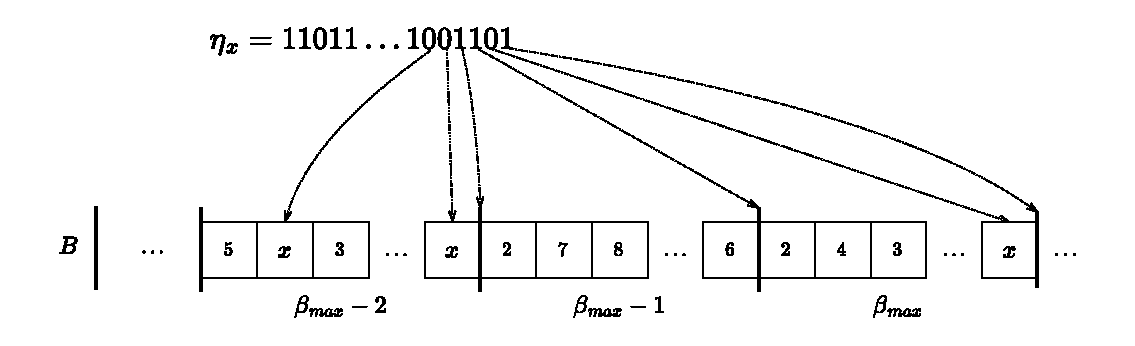
\includegraphics[scale=0.7]{figures/example_figure6.pdf}
        \caption{
            Example of a string $\eta_x$ over an array $B$. The array $B$ is depicted as being separated into small blocks. 
            The small blocks $\beta_{max}-2$, $\beta_{max}-1$, $\beta_{max}$ are depicted, considering that $\beta_{max}$ is the right most small block s.t. $x\in H_{\beta_{max}}$.
            For string $\eta_x$, each bit with value $0$ corresponds to an occurence of $x$, and each bit with value $1$ corresponds to the right border of some small block.
            }
        \label{fig:fig6}
    \end{figure}


    For each block $\beta$, we can store each set $H_{\beta}$ as an ordered array of pairs of integers $(x, p_x)$, $x$ representing the element of $H_{\beta}$ which is being stored, and $p_x$ is a pointer to the 
    data structure storing the string $\eta_x$.
    
    As, for each small block $\beta$, $|z_{\beta}|=O(\sqrt{n\cdot w})$ and $b=O(\sqrt{n\cdot w})$  the total space needed to store the strings $z_{\beta}$ will be:
    \[
        \sum_{\beta=1}^{b} |z_{\beta}| = O(\sqrt{n\cdot w}) \cdot O(\sqrt{n\cdot w}) = O(n \cdot w) \text{ bits }
    \]

    $O(n\cdot w)$ bits will be needed to store the strings $z_{\beta}$, thus, $O(n)$ words of RAM will be stored.
    
    As for each small block $\beta$, $|H_{\beta}|=O(\sqrt{n/w})$, the space needed to store the sets $H_{\beta}$ will be:

    \[
        \sum_{i=1}^{b} | H_{i} | = O( \sqrt{n/w} ) \cdot O( \sqrt{n\cdot w} ) = O(n) \text{ words of RAM. }
    \]


    For each string $\eta_x$, let $\beta_{\text{max}}$ be the rightmost small block that contains $x$, let the number of bits with value $0$, be $size_0(\eta_x)$, and the number of bits with value $1$ be $size_1(\eta_x)$.
    \[
        size_0(\eta_x)>\beta_{\text{max}} , size_1(\eta_x)=\beta_{\text{max}} \implies size_0(\eta_x)>size_1(\eta_x)
    \]

    Thus, the space required to store the strings $\eta_x$ will be:

    \[
        \sum_{x \in ( \cup_{\beta=1}^{b}H_{\beta} ) } |\eta_x| = \sum_{x \in ( \cup_{\beta=1}^{b}H_{\beta} ) } size_0(\eta_x)+size_1(\eta_x)  
    \]
    \[
        \leq  \sum_{x \in ( \cup_{\beta=1}^{b}H_{\beta} ) } 2\cdot size_0{\eta_x} \leq  \sum_{x \in ( \cup_{\beta=1}^{b}H_{\beta} ) } \textbf{freq}_x(1,n)
    \]
    \[
        =O(n) \text{ bits of space.}
    \]

    Thus, for maintaining the strings $\eta_x$, we need $O(n/w)=o(n)$ words of RAM.

    Finally, we may state that the total space required by this data structure is $O(n)$.

    \subsubsection{Query Algorithm.} The  query algorithm is as follows:
    \begin{enumerate}
        \item[] Given the interval $[i,j]$: 
        
        \item We determine the rightmost big block $\beta'$, of size $\beta'$, which intersects $[i,j]$. As the length of the prefix of $B$, covered with big blocks $1$ through $\beta'$, is :
            \[
             \sum_{k=1}^{\beta'}k=\frac{\beta'\cdot(\beta'+1)}{2} \leq 2 \cdot j 
            \] 
            We can obtain:
            \[
                \beta'^2 \leq 2\cdot ( \frac{\beta'\cdot(\beta'+1)}{2} ) \leq 4\cdot j \implies \beta' = O(\sqrt{j}) 
            \]

        Afterwards, we determine the leftmost and the rightmost small blocks, $\beta_1$ and $\beta_2$, respectively, that are fully contained in the interval $[i,j]$. Note that:
        \[
            size(\beta_1)\leq size(\beta_2)
        \]
        \[
            size(\beta_2) = \beta'/\sqrt{w} = O(\sqrt{j/w})
        \]
        
        If there are no small blocks that are fully contained in the interval $[i,j]$, then we can just iterate through  all the elements of $[i,j]$ and determine the range mode, 
        which will take $O(\sqrt{j/w})$ time.

        \item   Let $l_1$ be the left endpoint of the small block $\beta_1$ and $r_2$ be the right endpoint of the small block $\beta_2$ in array $B$.        
                We query the string $z_{\beta_2}$, and get the values $p_2=|z_{\beta_2}|$, and $p_1=\textbf{select}_{1}(z_{\beta_2}, \beta_1)$ 
                corresponding to the left endpoint of the small block $\beta_1$. 
                Further, we calculate:
                \[
                    f = ( p_2 - p_1 )-( \beta_2 - \beta_1 )
                \] 
                which corresponds to $f=\min( \phi(  l_1, r_2 ), \beta_2)$.

                In order to get an element $x$, which has frequency at least $f$ in the interval of small blocks $[\beta_1, \beta_2]$, we can get the rightmost position $p_f$, 
                corresponding to the left end of the small block $\beta_f$, such that, there are exactly $f$ bits with value $0$ in the interval $[p_f, p_2]$ in the string $\eta_x$. 
                This can be done easily, using $\textbf{rank}$ and $\textbf{select}$ 
                operations, as stated by Chan et al.\cite{chan2014linear}. Then, we need to iterate 
                through each position $k$ of the small block $\beta_f$, and check whether there are at least $f$ occurrences of $B_k$ inside the interval of small blocks $[ k , r_2 ]$.

        \item Further, we iterate through the elements $x$ of $H_{\beta_2+1}$, and find the values of their frequencies in the interval of small blocks $[\beta_1,\beta_2]$.
              In order to find the frequency of element $x$ in the interval of small blocks $[\beta_1, \beta_2]$, we query the string $\eta_x$ for values:
              \[
                    p_1=\textbf{select}_1(\eta_x,\beta_1-1)
              \]
              \[
                    p_2 = \textbf{select}_1(\eta_x, \beta_2 )
              \]
            $p_1$ being the position of the bit with value $1$ in string $\eta_x$, corresponding to the right endpoint of the small interval $\beta_1-1$, and $p_2$, being the position 
            of the bit with value $1$, corresponding to the right endpoint of the small interval $\beta_2$.
            Thus, the  frequency of the element $x$ will be:
            \[
                f_x=(p_2-p_1)-( \beta_2-\beta_1+1 )
            \]
            Further, we update the value of $f$ the following way: 
            \[
                f := \max(f, \max_{x \in H_{\beta_2+1}}(f_x) )
            \]

            This way, in a manner similar to that presented in $\textbf{lemma 1}$ and $\textbf{lemma 2}$, we obtain the value $\phi( l_1, r_2 )$, 
            which is exactly the frequency of a mode, in the interval corresponding to the small blocks $\{\beta_1, \beta_1+1,\dots,\beta_2 \}$. We must note, that during this step, it is also easy 
            to keep track of an element $x$ of maximum frequency.

        \item Now, we must iterate through positions $k \in ( [i,j] \setminus [l_1, r_2] ) $ and try to increase the frequency $f$, using the arrays 
            $Q$, $B$ and $Q^{-1}$, as in $\textbf{lemma 1}$ and $\textbf{lemma 2}$. This will take at most $O(\sqrt{j/w})$ time, which is an upper bound on the sizes of the small blocks $\beta_1$ and $\beta_2$.
        
        

    \end{enumerate}

    \subsubsection{Analysis.}
    This query algorithm will clearly require $O(\sqrt{j/w})$ time, as step 2 takes at most $O(\sqrt{j/w})$ time, step $3$ takes at most $O(\sqrt{ r_2/w } )=O(\sqrt{j/w})$ time, 
    and step $4$ similarly, takes at most $O(\sqrt{j/w})$ time. $\qed$



    \begin{algorithm}[H]
        \caption{Lemma 3 Query Algorithm}\label{lemma3Query}
        \begin{algorithmic}[1]
        \Function{Query}{}
        
        \Comment{Step 1:}

        \State $\beta'\gets \lceil -\frac{1}{2} + \sqrt{ \frac{1}{4} + 2 \cdot j } \rceil$
        
        \State $\beta_2 \gets \lfloor \frac{(j-\frac{ \beta'(\beta'-1) }{2})}{ \frac{\beta'}{\sqrt{w}} } \rfloor + (\beta'-1) \cdot \sqrt{w} $
        
        \State $t \gets \lceil -\frac{1}{2} + \sqrt{ \frac{1}{4} + 2 \cdot i } \rceil$
        \State $v \gets \lfloor \frac{(i-\frac{ t(t-1) }{2})}{ \frac{t}{\sqrt{w}} } \rfloor + (t-1) \cdot \sqrt{w} $
        \State $\beta_1 \gets v+2$
        \If{ $ (v - (t-1) \cdot \sqrt{w}) \cdot \frac{t}{\sqrt{w}}+\frac{t\cdot (t-1)}{2} + 1 = i $ }
            \State $\beta_1 \gets v+1$
        \EndIf

        \If {$\beta_1>\beta_2$}
        \State \#Iterate through each element of [i,j] and return the answer.
        
        \EndIf

        \Comment{Step 2:}
        
        \State $l_1 \gets (\beta_1-1 - (t-1) \cdot \sqrt{w}) \cdot \frac{t}{\sqrt{w}}+\frac{t\cdot (t-1)}{2}+1$
        \State $r_2 \gets (\beta_2 - (\beta'-1) \cdot \sqrt{w}) \cdot \frac{\beta'}{\sqrt{w}}+\frac{\beta'\cdot (\beta'-1)}{2}$
        
        \State $p_2 \gets |z_{\beta_2}|, p_1\gets \textbf{select}_1(z_{\beta_2}, \beta_1)$

        \State $f \gets f = ( p_2 - p_1 )-( \beta_2 - \beta_1 )$ 
        \State \# Find $\beta_f$ and $p_f$, and iterate through the block $\beta_f$, and get the candidate element $m$.

        \Comment{Step 3:}

        \For{$x\in H_{\beta_2+1}$}
            \State $p_1^x=\textbf{select}_1(\eta_x,\beta_1-1)$

            \State $p_2^x = \textbf{select}_1(\eta_x, \beta_2 )$
          
            \State $f_x\gets (p_2^x-p_1^x)-(\beta_2-\beta_1+1)$
            
            \If{$f_x>f$}
            \State $f\gets f_x$
            \State $m\gets x$
            \EndIf
            \EndFor
        

        \Comment{Step 4:}
        
        \For{$k \in [i,l_1-1]$}
            \While{$Q_{B_{k}}( Q^{-1}(k)+f+1 )\leq j$}
                \State $f\gets f+1$
                \State $m\gets B_k$
            \EndWhile
        \EndFor
    
        \For{$k \in [r_2+1,j]$}
            \While{$Q_{B_{k}}( Q^{-1}(k)-f-1 )\geq i$}
                \State $f\gets f+1$
                \State $m\gets B_k$
            \EndWhile
        \EndFor
    
        \Return $(C(m),f)$
    
        \EndFunction
        \end{algorithmic}
    \end{algorithm}

\end{proof}


\begin{theorem}
    Given an array $A[1:n]$, there exists a data structure, requiring $O(n)$ words of RAM, that supports 
    range mode queries over an interval $[i,j]$ in time $O(\min ( \sqrt{j-i+1}, \sqrt{j/w} ) )$.    
\end{theorem}
\begin{proof}
    Firstly, we will build the arrays $B$, $C$, $Q$, $Q^{-1}$ and the set $D$, which will take $O(n\log n)$ time and $O(n)$ space.
    Further, we will build an instance of the data structure defined in \textbf{lemma 3}, denoted by $DS_1$, and an instance of the data structure defined in \textbf{theorem 1}, denoted by $DS_2$.
    The arrays, as well as both of the instances of the data structures mentioned above, will require $O(n)$ space, thus, the space required by the current data structure is $O(n)$.
    
    \subsubsection{Query Algorithm.} The query algorithm is as follows:
    \begin{enumerate}
        \item[] Given the interval $[i,j]$:
        
        \item Estimate the time required by a query over the data structure $DS_1$ and the interval $[i,j]$. Let this time estimation be $t_1$. 
              Estimate the time required by a query over the data structure $DS_2$ and the interval $[i,j]$. Let this time estimation be $t_2$. 
        
        \item If $t_1<t_2$, then, return $DS_1.query(i,j)$, otherwise, return $DS_2.query(i,j)$.      
    
    \end{enumerate}

    \subsubsection{Analysis.}
    It is easy to do the time estimates $t_1$ and $t_2$ up to a constant factor, in at most logarithmic time.
    
    Thus, the runtime of the query algorithm is $O(\min ( \sqrt{j-i+1}, \sqrt{j/w} ) )$.$\qed$

\end{proof}


\section{Adding Elements at the End of the Array}

Further, considering the fact, that we can implement a compact, data structure, supporting rank/select operations in $O(1)$ time, and adding a bit to the 
end of the array in amortyzed $O(1)$ time, we will show how to make the data structure from section $2$ support adding an element at the end of the 
array $A[1:n]$ in amortyzed $O(\sqrt {n \cdot w} )$ time, while requiring linear space and keeping the same query time.



\begin{lemma}
    Given an array $A[1:n]$, there exists a data structure, that respects the same conditions as the data structure constructed in 
    Lemma $1$, and also supports adding an element at the end of the array $A[1:n]$, in amortyzed $O(\sqrt{2^L})$ time.

\end{lemma}
\begin{proof}
    As the only data stored in the data structure from $\textbf{lemma 1}$, are the strings $s^L_{\beta_1}$, we will present an algorithm to update $s^L_{\beta_1}$, 
    as new elements are added to the end of array $A$.
    
    \subsubsection{Update Algorithm.}
    Suppose that there are $\beta'$ big blocks of size exactly $b_L'=2^L$ that are fully contained in array $B[1:n]$. 
    Let $\beta$ be the number of small blocks, of size $b_L=\sqrt{2^L}$, that are fully contained in the array $B[1:n]$. 
    Let $\beta_{new}=\beta+1$ be the new small block, which is constructed as new elements are appended to the end of $A[1:n]$.


    
    \begin{enumerate}
        \item[] An update is given, in the form of a number $x$, that must be added to the end of $A[1:n]$.
        
        \item Determine the element $y$ of array $B$, s.t. $C_{y}=x$, then add $n+1$ to the end of $Q_{y}$, and add $|Q_{y}|$ to the end of $Q^{-1}$.
        If such an element $y$ does not exist, then, $\Delta := \Delta+1$ and $y:=\Delta$, 
        add $x$ to the end of the array $C$, define $Q_{y}=\{n+1\}$, and add $1$ to the end of $Q^{-1}$. Add $y$ to the end of $B$. 
        
        \item 
        For each small block $\beta_i\in \{ \beta_{new}-\sqrt{2^L}+1, \dots , \beta_{new} \}$, let $l_i$ be the left endpoint of $\beta_i$. 
        We must check, whether the new element $y$ added to $B[1:n]$, changes the maximum frequency 
        inside the interval of small blocks $[\beta_i, \beta_{new}]$, by verifying the following condition:
        \[
            p=|s^{L}_{\beta_i}|, c_1 = \textbf{rank}_1(s^{L}_{\beta_i}, p)
        \]
        \[
            f=p-c_1, l_y = Q_{y}( Q^{-1}(n+1)-f-1 )
        \]
        \[
            l_y \geq l_i \text{ and } f+1\leq \sqrt{2^L}
        \]

        If this condition holds, then we add a bit with value $0$ to the end of $s^L_{\beta_i}$. This will signify 
        the increase in the maximum frequency of an element, recorded by the string $s^{L}_{\beta_i}$. We must also note, that the strings $s^{L}_{\beta_i}$ will change 
        their structure during these intermediary frequency-increase steps, as bits with value $0$ will be present at the end of $s^{L}_{\beta_i}$. 
        This will not influence the queries over $s^{L}_{\beta_i}$ required by the data structure from $\textbf{lemma 1}$.

        \item If the position $n+1$ is the right endpoint of a new small block $\beta_{ \text{new} }$ that is now fully contained in array $B[1:(n+1) ]$, 
        then, for each $\beta_i\in \{ \beta_{new}-\sqrt{2^L}+1, \dots , \beta_{new} \}$,  we must update the information stored in $s^L_{\beta_i}$. 
        In such a case, we must add $1$ to the end of $s^L_{\beta_i}$, which will signify the addition of a right endpoint of a new full small block.  
        
        \item Finally, we add element $x$ to the end of array $A$, and set $n:=n+1$.

    \end{enumerate}

    \subsubsection{Analysis.}
    It is easy to see that the first step takes at most logarithmic time. The second step, will take amortyzed $O(\sqrt{2^L})$  time, as there may be at most $O(\sqrt{2^L})$ small blocks $\beta_i$, 
    and each append of a bit to the end of $\beta_i$ takes amortyzed $O(1)$ time. Similarly, the third step takes $O(\sqrt{2^L})$ time.

    The required space will still remain linear, as $s^L_{\beta_1}$ has been proven to require $O(n/w)$ words of $RAM$, and $O(1)$ more bits of space will be added at each update. $\qed$

    \begin{algorithm}[H]
        \caption{Lemma 4 Update Algorithm}\label{lemma4Update}
        \begin{algorithmic}[1]
        \Function{Update}{}
        
        \Comment{Step 1:}
        
        \State $y\gets 0$

        \If{$x\notin D$}
        
        \State $\Delta\gets \Delta+1$
        \State $y\gets \Delta$
        \State $D.insert(x)$
        \State $Q_{y}\gets \{n+1\}$
        \State $Q^{-1}.append(1)$

        \Else{}
        
        \State $y \gets D.rank(x)$
        \State $Q_{y}.append(n+1)$
        \State $Q^{-1}.append(|Q_{y}|)$

        \EndIf

        \State $B.append(y)$

        \Comment{Step 2:}

        \For{$\beta_i\in\{ \beta_{new}-\sqrt{2^L}+1, \dots , \beta_{new} \}$}
            
        \State $p=|s^{L}_{\beta_i}|, c_1 = \textbf{rank}_1(s^{L}_{\beta_i}, p)$
        \State $f=p-c_1, l_y = Q_{y}( Q^{-1}(n+1)-f-1 )$
        
        \If{$l_y \geq l_i \text{ and } f+1\leq \sqrt{2^L}$}
            \State $s^L_{\beta_i}.append(0)$
        \EndIf
        
        \EndFor

        \Comment{Step 3:}
        \If{$i$ is the right endpoint of $\beta_{new}$}
            \For{$\beta_i\in\{ \beta_{new}-\sqrt{2^L}+1, \dots , \beta_{new} \}$}
                \State $s^L_{\beta_i}.append(1)$
            \EndFor
        \EndIf

        \Comment{Step 4:}

        \State $A.append(x)$
        \State $n\gets n+1$
        
        \EndFunction
        \end{algorithmic}
    \end{algorithm}
    

\end{proof}


\begin{lemma}
    Given an array $A[1:n]$, there exists a data structure, that respects the same conditions as the data structure constructed in 
    Lemma $2$, and also supports adding an element at the end of the array $A[1:n]$, in amortyzed $O(\sqrt{2^L})$ time.

\end{lemma}
\begin{proof}
    As the only additional data stored in the data structure from $\textbf{lemma 2}$, are the sets $F^L_i$ and the strings $Y^L_{i,x}$, 
    we will present an algorithm to update them, as new elements are added to the end of array $A$.

    \subsubsection{Update Algorithm.}
    Suppose that there are $\beta'$ big blocks of size exactly $b_L'=2^L$ that are fully contained in array $B[1:n]$. 
    Let $\beta$ be the number of small blocks, of size $b_L=\sqrt{2^L}$, that are fully contained in the array $B[1:n]$. 
    Let $\beta_{new}=\beta+1$ be the new small block, which is constructed as new elements are appended to the end of $A[1:n]$, 
    and $\beta_{new}'=\beta'+1$ be the new big block, which is constructed as new elements are appended to the end of $A[1:n]$.

    \begin{enumerate}
        \item[] An update is given, in the form of a number $x$, that must be added to the end of $A[1:n]$.
        
        \item Determine the element $y$ of array $B$, s.t. $C_{y}=x$, then add $n+1$ to the end of $Q_{y}$, and add $size(Q_{y})$ to the end of $Q^{-1}$.
        If such an element $y$ does not exist, then, $\Delta := \Delta+1$ and $y:=\Delta$, 
        add $x$ to the end of the array $C$, define $Q_{y}=\{n+1\}$, and add $1$ to the end of $Q^{-1}$. Add $y$ to the end of $B$. 
        
        \item We must first check, if the frequency of the element $y$ in the interval of $B$, 
        corresponding to the interval of big blocks $[\beta', \beta'_{new}]$ is $>\sqrt{2^L}$. 
        According to Chan et al.\cite{chan2014linear}, this can be done in $O(\log n)$ time, using the arrays $Q_{y}$ and $Q^{-1}$.

        If the frequency of $y$ is not big enough, then we can stop the update procedure.

        Otherwise, we must check whether the element $y$ is present in $F^L_{\beta'}$. 
        This can be done simply, by iterating through the elements of $F^L_{\beta'}$. 

        If $y$ is present in $F^L_{\beta'}$, then we must add $0$ to the end of $Y^L_{\beta', y}$.
        Otherwise, we must create the string $Y^L_{\beta', y}$, and add the pair $(y, p_y)$ to the end of $F^L_{\beta'}$.
        
        \item In this step, we will present a procedure, to create the string $Y^L_{\beta', y}$ 
        when $y$ has to be added to the set $F^L_{\beta'}$ for the first time.
            \begin{enumerate}
                \item Create the string $Y_{\beta', y}^L$, and the pointer $p_y$.
                \item 
                Let $p$ be the leftmost position, s.t. $B_p=y$, in the interval of $B$, corresponding to the interval of big blocks $[\beta',\beta_{new}']$.
                Let $\beta_p$ be the small blocks that contains the position $p$. 
                These two values can be found trivially in $O(\sqrt{2^L})$ time.
                
                Let $\beta_{first}$, be the leftmost small block, that is contained in the big block $\beta'$.
                We insert $\beta_{p}-\beta_{first}$ bits with value $1$ to the end of $Y_{\beta', y}^L$.
                Note that $\beta_{p}-\beta_{first}=O(\sqrt{2^L})$.
                \item  
                    Insert a bit with value $0$ to the end of $Y_{\beta', y}^L$.
                    If $p=n+1$, it means that we have evaluated currently the last position at which the value $y$ can be found in $B$, and we must stop the construction procedure.
                    Set $p:=Q_{y}( Q^{-1}(p)+1 )$.
                    If $p$ is outside of the small block $\beta_p$, then, set $\beta_p:=\beta_p+1$, 
                    and insert a bit with value $1$ to the end of $Y_{\beta', y}^L$.
                \item Go to step (c).
            \end{enumerate}
        
        \item In a manner similar to steps $2$ and $3$, we update, or create if not found, the string $Y_{\beta_{new}', y}^{L}$ and the set $F_{\beta_{new}'}^L$.
        
        \item Further, we check whether the current position is the  rightmost position contained in 
        the big block $\beta'$. If this is true, and the string $Y_{\beta', y}^L$ exists, then we add a bit with value $1$ to the end of $Y_{\beta', y}^L$.
        In the same way, if $n+1$ is the rightmost position of the big block $\beta_{new}'$ and the string $Y_{\beta_{new}', y}^L$ exists, then we add a bit with value $1$ to the end of $Y_{\beta_{new}', y}^L$.
            
        \item As a final step, we append element $x$ to the end of array $A$, and set $n:=n+1$.
    \end{enumerate}

    \subsubsection{Analysis.}
    It is easy to see that the first step takes at most logarithmic time. The second step takes at most $O(\sqrt{2^L})$ amortyzed time.
    The procedure described in step $3$, takes $O(\sqrt{2^L})$ time, as we begin iterating through the positions of $y$, 
    only the first time, when the frequency of $y$ relative to the big blocks $\beta'$ and $\beta_{new}'$ increases beyond $\sqrt{2^L}$. 
    Thus, in step $3$, we chekc only $O(\sqrt{2^L})$ positions of $y$, and at most $O(\sqrt{2^L})$ small blocks, thus, we need only $O(\sqrt{2^L})$ amortyzed time.
    The $4$-th step is similar to the  $2$-nd step followed by the $3$-rd one, thus it takes $O(\sqrt{2^L})$ amortyzed time. The last step takes amortyzed $O(1)$ time.
    
    Thus, the update algorithm runs in $O(\sqrt{2^L})$ amortyzed time.$\qed$ 
    
    \begin{algorithm}[H]
        \caption{Lemma 5 Update Algorithm}\label{lemma5Update}
        \begin{algorithmic}[1]

        \Function{Update}{}
        
        \Comment{Step 1:}
        
        \State $y\gets 0$

        \If{$x\notin D$}
        
        \State $\Delta\gets \Delta+1$
        \State $y\gets \Delta$
        \State $D.insert(x)$
        \State $Q_{y}\gets \{n+1\}$
        \State $Q^{-1}.append(1)$

        \Else{}
        
        \State $y \gets D.rank(x)$
        \State $Q_{y}.append(n+1)$
        \State $Q^{-1}.append(|Q_{y}|)$

        \EndIf

        \State $B.append(y)$

        \Comment{Step 2,3:}

        \If{the frequency of y is $>\sqrt{2^L}$ in the interval of big blocks $[\beta', \beta'_{new}]$}
            \If{$y\in F_{\beta'}^L$}
                \State $Y_{\beta', y}^L.append(0)$
            \Else{}
                \State $(Y_{\beta', y}^L, p_y) \gets buildY(\beta', y, L) $
                \State $F_{\beta'}^L.insert(y)$
            \EndIf
        \EndIf

        \Comment{Step 4:}

            \If{the frequency of y is $>\sqrt{2^L}$ in the interval of big block $\beta'_{new}$}
                \If{$y\in F_{\beta'_{new}}^L$}
                    \State $Y_{\beta'_{new}, y}^L.append(0)$
                \Else{}
                    \State $(Y_{\beta'_{new}, y}^L, p_y) \gets buildY(\beta'_{new}, y, L) $
                    \State $F_{\beta'_{new}}^L.insert(y)$
                \EndIf
            \EndIf
        

        \Comment{Step 5:}

        \If{$n+1$ is the right endpoint of the big block $\beta'_{new}$}
            \If{ $Y_{\beta', y}^L$ exists }
                \State $Y_{\beta', y}^L.append(1)$
            \EndIf
            \If{ $Y_{\beta'_{new}, y}^L$ exists }
                \State $Y_{\beta'_{new}, y}^L.append(1)$
            \EndIf
        \EndIf

        \Comment{Step 6:}
        \State $A.append(x)$
        \State $n\gets n+1$
        
        \EndFunction
        \end{algorithmic}
    \end{algorithm}

    \begin{algorithm}[H]
        \caption{Lemma 5 Algorithm for building $Y_{\beta', y}^L$}\label{lemma4Build}
        \begin{algorithmic}[1]
        
        \Function{buildY}{$\beta', y, L$}
            \State Create $Y_{\beta', y}^L$ and the pointer $p_y$
            \State Let $p$ be the leftmost position in $B$ of the element $y$, in the interval of blocks $[\beta', \beta'_{new}]$
            \State $\beta_p \gets \lfloor (p+\sqrt{2^L})/\sqrt{2^L} \rfloor$
            \State $\beta_{first} \gets (\beta'-1)\cdot \sqrt{2^L} + 1 $
            
            \For{$k \in [1, \beta_p-\beta_{first}]$}
                \State $Y_{\beta', y}^L.append(1)$
            \EndFor


            \While{$p<n+1$}
                \State $Y_{\beta', y}^L.append(0)$
                \State $p\gets Q_{y}( Q^{-1}(p)+1 )$
                \If{$p$ is outside the small block $\beta_p$}
                    \State $\beta_p \gets \beta_p+1$
                    \State $Y_{\beta', y}^L.append(1)$
                \EndIf
            \EndWhile
            \Return $(Y_{\beta', y}^L, p_y)$
            \EndFunction
        \end{algorithmic}
    \end{algorithm}

    


\end{proof}

Further, we will summarize the results from $\textbf{lemma 4}$ and $\textbf{lemma 5}$ and show how to achieve amortyzed $O(w+\sqrt{n})$ runtime for updates, while keeping the other properties for the data structures described in $\textbf{lemma 1}$ and \textbf{lemma 2}.
\begin{theorem}
    Given an array $A[1:n]$, there exists a data structure, requiring arrays $B$, $C$, $Q$, and additional $O(n)$ words of RAM, that supports 
    range mode queries over an interval $[i,j]$ in $O(\sqrt{j-i+1})$ time, and supports adding an element at the end of $A[1:n]$ in amortyzed $O(w+\sqrt{n})$ time.
\end{theorem}
\begin{proof}
    As declared in \textbf{lemma 4} and \textbf{lemma 5}, the data structures from \textbf{lemma 1} and \textbf{lemma 2} 
    can be modified in order to support updates in $O(\sqrt{2^L})$ time, 
    while requiring the same amoung of space and maintaining a query in $O(\sqrt{2^L})$ time.
    
    Further, for each $L\in \{0,\dots,\lceil \log n \rceil\}$, we will build an instance of the data structure described in \textbf{lemma 4}, denoted by $DS_1^L$, and an instance of the data structure 
    described in \textbf{lemma 5}, denoted by $DS_2^L$. These instances will take $O(n)$ space, as the arrays $B$, $C$, $Q$, $Q^{-1}$, $F^L_{i}$ and the set $D$, will be shared among them, and the additional information 
    will take $O(\log n \cdot n/w) = O(n)$ space.
    
    As the query time remains unchanged, we must study only the update time. As for one update, at a moment in time when the array $A$ has length $n$, 
    for each $L\in \{0,\dots,\lceil \log n \rceil\}$ the update time if $O(\sqrt{2^L})$, the total update time for all $L\in \{0,\dots,\lceil \log n \rceil\}$, $DS_1^L$ and $DS_2^L$  will be:
    \[
        \sum_{L=0}^{\lceil \log n \rceil}\lceil \sqrt{2^L} \rceil \leq w + \sqrt{n} \cdot \sum_{L=0}^{\lceil \log n \rceil} \frac{1}{\sqrt{2^L}}
        \leq \sqrt{n} \cdot \sum_{L=0}^{\inf} \frac{1}{\sqrt{2^L}}   
     \]
     \[   
        \leq w + O(\sqrt{n}) = O(w+\sqrt{n})  \qed
     \]
\end{proof}

\begin{lemma}
    Given an array $A[1:n]$, there exists a data structure requiring $O(n)$ words of RAM, that supports 
    range mode queries over an interval $[i,j]$ in $O( \sqrt{j/w}  )$ time, and supports adding an element at the end of $A[1:n]$ in amortyzed $O(\sqrt{n \cdot w})$ time. 
\end{lemma}
\begin{proof}
    As the only additional data stored in the data structure from $\textbf{lemma 3}$, are the sets $H_{\beta}$ and the strings $z_{\beta}$ and $\eta_x$, 
    we will present an algorithm to update them, as new elements are added to the end of array $A$.
    
    Firstly, we suppose there are $\beta'$ big blocks, fully contained in array $B[1:n]$, 
    and $\beta$ be the number of small blocks fully contained in array $B[1:n]$.
    Let $\beta_{new} = \beta+1$ be the new small block, constructed while new elements are appended to $A$,
    and, similarly, let $\beta_{new}'=\beta'+1$ be the new big block constructed while new elements are appended to $A$.                


    In our approach, we also introduce the array $\tau$ of size $\beta_{new}$, defined below:
    \begin{definition}
        Let array $\tau$, be an array of integers, of size $\beta_{new}$, obeying the following properties:
        \begin{property}
            For each small block $k \in \{1,\dots , \beta_{new}$ \}, having $l_k$ as its left endpoint:
            \[
            \tau_k = \phi(l_k, n)
            \] 
        \end{property}
    \end{definition}

    In other words, in $\tau$, we will store a decreasing array, describing the frequency 
    of the most frequent element in the last small blocks of the array $B$.

    \subsubsection{Update Algorithm.} 
    
    \begin{enumerate}
        \item[] An update is given, in the form of a number x, that must be added to the
        end of A[1 : n].
        
        \item Determine the element $y$ of array $B$, s.t. $C_{y}=x$, then add $n+1$ to the end of $Q_{y}$, and add $size(Q_{y})$ to the end of $Q^{-1}$.
        If such an element $y$ does not exist, then, $\Delta := \Delta+1$ and $y:=\Delta$, 
        add $x$ to the end of the array $C$, define $Q_{y}=\{n+1\}$, and add $1$ to the end of $Q^{-1}$. Add $y$ to the end of $B$. 
        
        \item In this step, we will iterate through each position $k$ in $\tau$, and check whether we can increase $\tau_k$. 
                We will use the fact, that the addition of the element $y$ to the end of $B$, will increase each value stored in $\tau$ by at most $1$, because, 
                for each $k$, $\phi(l_k, n+1)\leq 1+\phi(l_k, n)$.

                This procedure is summarized in the following sub-steps:
                
                \begin{enumerate}
                    \item Let $\beta_{current}:=\beta_{new}$. 
                    \item Let $l_{\beta_{current}}$ be the left endpoint of the small block $\beta_{current}$.
                    \item If $Q_{y}( |Q_{y}|-\tau_{\beta_{current}} )\geq l_k$, then set $\tau_{\beta_{current}}:=\tau_{\beta_{current}}+1$.
                    \item If $\beta_{current}>1$, set $\beta_{current}:=\beta_{current}-1$, and go back to step (b).

                \end{enumerate}

                This way, we update the values of $\tau$, in $O(\beta_{new})$ time.
        
        \item If $y\in H_{\beta_{new}}$, then, we add a bit with value $0$ to the end of $\eta_{y}$. 
        Otherwise, we check if $ \textbf{freq}_{y}(1, n)>\beta_{new} $. If this is true, then we will add $y$ to $H_{\beta_{new}}$, and update the string $\eta_{y}$. If $\eta_{y}$ did not exist, we will suppose that it was empty.
        
        We descrive the process of updating the string $\eta_{y}$, by the following procedure:
                \begin{enumerate}
                    \item Let $\beta_{current}:=\textbf{rank}_{1}(\eta_{y}, |\eta_{y}|)$, 
                    $p:=\textbf{rank}_{0}(\eta_{y}, |\eta_{y}|)+1$, where $\beta_{current}$ will represent the current small block, 
                    and $p$ will represent the position in array $Q_y$, of the first position of $y$ that has not been considered in the string $\eta_{y}$ yet.
                    \item Let $r_{current}$ be the right endpoint of the small block $\beta_{current}$.
                    \item If $p\leq r_{current}$, then, set $p:=p+1$, add $0$ to $\eta_{y}$, and return to step $3.b$.
                    \item If $\beta_{current}<\beta_{new}$, then set $\beta_{current}:=\beta_{current}+1$, add $1$ to the end of $\eta_{y}$ and go back to step $3.b$.
                \end{enumerate}
        
        \item If the position $n+1$ is the right endpoint of the small block $\beta_{new}$, then we iterate through each $y\in H_{\beta_{new}}$ and add $1$ to the end of $\eta_{y}$.
        
        \item If the position $n+1$ is the right endpoint of the small block $\beta_{new}$, then, for each $y \in H_{\beta_{new}}$ , if it has frequency $\geq\beta_{new}+1$, 
        add $y$ to $H_{\beta_{new}+1}$.
        
        \item If the position $n+1$ is the right endpoint of the small block $\beta_{new}$, then we have to build $z_{\beta_{new}}$, by using the array $\tau$. 
        
        We will describe the process of constructing $z_{\beta_{new}}$, by the following procedure:
        \begin{enumerate}
            \item Let $k:=\beta_{new}$, and $f:=0$.
            \item If $f < \min(\tau_{k}, \beta_{new})$, then, set $f:=f+1$, add $0$ to the end of $z_{\beta_{new}}$ and return to step $5.b$.
            \item If $k>0$, add $1$ to the end of $z_{\beta_{new}}$, set $k:=k-1$ and go to step $5.b$.
            \item Now, we will reverse the string $z_{\beta_{new}}$, in order to make it obey the definition declared in $\textbf{lemma 3}$.
        \end{enumerate}

        Now, we will set $\beta_{new}:=\beta_{new}+1$, s.t. $\beta_{new}$ will now have the value of the small block, that will begin its construction when 
        an element will be append to $B$ at position $n+2$. Also, we will append a new integer with value $0$ to the end of $\tau$.

        

        \item Finally, we append $x$ to $A$, and set $n:=n+1$.
    \end{enumerate}

    \subsubsection{Analysis.}
    
    It is easy to see that the first step takes at most logarithmic time. \item If the position $n+1$ is the right endpoint of the small block 
    The second step will take $O(\beta_{new})=O(|\tau|)=O(\sqrt{n\cdot w})$ time.

    The third step will take at most $O(\beta_{new})=O(\sqrt{n\cdot w})$ time, because, if $y$ was already in $H_{\beta_{new}}$, then we need only $O(1)$ 
    time to update $\eta_y$, and if $y$ was not in $H_{\beta_{new}}$ yet, then the frequency of $y$ currently is at most $\beta_{new}+1$, and the construction of 
    $\eta_{y}$ will take at most $O(\beta_{new})=O(\sqrt{n\cdot w})$ time.

    The fourth step will take at most $O(\sqrt{n/w})$ time, as well as the fifth step, as we will just need to iterate through each element $y\in H_{\beta_{new}}$, 
    and $|H_{\beta_{new}}|=O(\sqrt{n/w})$.

    The sixth step will take $O(\sqrt{n\cdot w})$ time, as we will iterate through the possible values of $f$ from $0$ to at most $\beta_{new}$, 
    and through each entry of $\tau$, and $O(\beta_{new}+|\tau|)=O(\beta_{new})=O(\sqrt{n\cdot w})$.
    
    The seventh step, will take $O(1)$ time. Thus, the update algorithm will require $O(\sqrt{n\cdot w})$ time, 
    and will keep the linear-space restriction for our data structure.$\qed$



    \begin{algorithm}[H]
        \caption{Lemma 6 Update Algorithm}\label{lemma6Update}
        \begin{algorithmic}[1]

        \Function{Update}{}
        
        \Comment{Step 1:}
        
        \State $y\gets 0$

        \If{$x\notin D$}
        
        \State $\Delta\gets \Delta+1$
        \State $y\gets \Delta$
        \State $D.insert(x)$
        \State $Q_{y}\gets \{n+1\}$
        \State $Q^{-1}.append(1)$

        \Else{}
        
        \State $y \gets D.rank(x)$
        \State $Q_{y}.append(n+1)$
        \State $Q^{-1}.append(|Q_{y}|)$

        \EndIf

        \State $B.append(y)$
        
        \Comment{Step 2:}
        \For{$\beta_{current} \in \{1,\dots,\beta_{new}\}$}
            \State Let $l_{\beta_{current}}$ be the left endpoint of the small block $\beta_{current}$ 
            \If{$Q_y( Q^{-1}(n+1)-\tau_{\beta_{current}}-1 ) \geq l_{\beta_{current}} $}
                \State $\tau_{\beta_{current}}\gets \tau_{\beta_{current}}+1$
            \EndIf
        \EndFor

        \Comment{Step 3:}

        \If{$\textbf{freq}_y(1,n)>\beta_{new}$}
            \If{$y \in H_{\beta_{new}}$}
                \State $\eta_y.append(0)$
            \Else{}
                \State $\eta_y \gets update\_\eta(y) $
                \State $H_{\beta_{new}}.insert(y)$
            \EndIf
        \EndIf

        \Comment{Steps 4,5,6:}

        \If{$n+1$ is the right endpoint of the small block $\beta_{new}$}
            \For{$y\in H_{\beta_{new}}$}
                \State $\eta_y.append(1)$
                \If{$\textbf{freq}_{y}(1, n)>\beta_{new}+1$}
                    \State $H_{\beta_{new}+1}.insert(y)$
                \EndIf
            \EndFor
            \State $z_{\beta_{new}} \gets build\_z(\beta_{new}, y)$
            \State $\beta_{new}\gets \beta_{new}+1$
            \State $\tau.append(0)$
        \EndIf

        \Comment{Step 7:}
        \State $A.append(x)$
        \State $n\gets n+1$
        
        \EndFunction
        \end{algorithmic}
    \end{algorithm}




    \begin{algorithm}[H]
        \caption{Lemma 6 Algorithm for updating/building $\eta_{y}$}\label{lemma6eta}
        \begin{algorithmic}[1]
        
        \Function{update\_$\eta$}{$y$}
            \If{$\eta_y$ does not exist}
                \State Create the string $\eta_y$
            \EndIf
            \State $\beta_{current}\gets \textbf{rank}_{1}(\eta_{y}, |\eta_{y}|)$ 
            \State $p\gets \textbf{rank}_{0}(\eta_{y}, |\eta_{y}|)+1$
            

            \While{$\beta_{current}<\beta_{new}$ or $( \beta_{current}=\beta_{new}  p\leq r_{current})$}
                \State Let $r_{current}$ be the right endpoint of the small block $\beta_{current}$
                
                \If{$p<r_{current}$}
                    \State $p\gets p+1$
                    \State $\eta_{y}.append(0)$
                \EndIf
                
                \State $\beta_{current}\gets \beta_{current}+1$
                \State $\eta_{y}.append(1)$
            \EndWhile

            \Return $\eta_{y}$
            \EndFunction
        \end{algorithmic}
    \end{algorithm}

    \begin{algorithm}[H]
        \caption{Lemma 6 Algorithm for building $z_{\beta_{new}}$}\label{lemma6z}
        \begin{algorithmic}[1]
        
        \Function{build\_z}{$\beta_{new}$}
            \If{$z_{\beta_{new}}$ does not exist}
                \State Create the string $z_{\beta_{new}}$
            \EndIf
            
            \State $f\gets 0$

            \For{$k \gets \beta_{new} \textbf{ downto } 1$}
                \While{$f < \min(\tau_k, \beta_{new})$}
                    \State $f\gets f+1$
                    \State $z_{\beta_{new}}.append(0)$
                \EndWhile
                \State $z_{\beta_{new}}.append(1)$
            \EndFor
            
            \State $z_{\beta_{new}}\gets reverse(z_{\beta_{new}})$


            \Return $z_{\beta_{new}}$
            \EndFunction
        \end{algorithmic}
    \end{algorithm}





\end{proof}


\begin{theorem}
    Given an array $A[1:n]$, there exists a data structure, requiring $O(n)$ words of RAM, that supports 
    range mode queries over an interval $[i,j]$ in $O(\min ( \sqrt{j-i+1}, \sqrt{j/w} ) )$ time, and supports adding an element at the end of $A[1:n]$ in amortyzed $O(w+\sqrt{n \cdot w})$ time.     
\end{theorem}
\begin{proof}



    Firstly, we will build the arrays $B$, $C$, $Q$, $Q^{-1}$ and the set $D$, which will take $O(n\log n)$ time and $O(n)$ space.
    Further, we will build an instance of the data structure defined in \textbf{lemma 6}, denoted by $DS_1$, and an instance of the data structure defined in \textbf{theorem 3}, denoted by $DS_2$.
    The arrays, as well as both of the instances of the data structures mentioned above, will require $O(n)$ space, thus, the space required by the current data structure is $O(n)$.
    
    Note that the time required by the query algorithm will remain the same as the runtime of the data structure defined in $\textbf{theorem 2}$, more exactly: 
    
    $O(\min(\sqrt{j-i+1}, \sqrt{j/w}) )$.

    The update algorithm will consist only of calling the methods $DS_1.update(x)$ and $DS_2.update(x)$, given an integer $x$ that will be appended to the end of $A$.
    Thus, the time required by the update algorithm for this data structure will be:
    \[
        O(w+\sqrt{n})+O(\sqrt{n\cdot w}) = O(w+\sqrt{n\cdot w}) \qed
    \]

\end{proof}

\section{Compact rank/select data structure}

We present a compact data structure, that supports $O(1)$ rank/select/access operations over a binary array $B$ of length $Z$, by using $O(Z)$ additional bits of space, and supports adding bits, one-by-one, at the end 
of array $B$ in amortyzed $O(1)$ time.


In the construction of our data structures, we will use the fact that we can implement an array for storing integers representable in a single word of RAM, that supports \textbf{access} operations in constant $O(1)$ time, and supports appending an integer to the end of the array in amortyzed $O(1)$ time, while requiring linear space.


Firstly, we will consider the following result:
\begin{lemma}
    There exists a data structure, that can store a binary array $B$ of size $Z$, by using $O(Z)$ bits, and will support $\textbf{rank}$ and $\textbf{access}$ operations in $O(1)$ time, 
    and appending a bit to the end of the array in amortyzed $O(1)$ time.
\end{lemma}
\begin{proof}
    Consider $w'=\lceil \frac{\log Z}{2} \rceil$. We will separate the array $B$ into adjacent blocks of size $w'$, and will represent each block, as a number stored as a word of RAM of size $w$.
    The array $B$, will be represented as an array of numbers $B'$, $B'_{i}$ containing the bits of the block $i$.
    
    We will build the array $P$, with size equal to that of $B'$, where each entry $P_i$ will be equal to the sum of bits with value $1$, in the blocks $1$ through $i$.    

    We will build a look-up table $T$, of size $O(2^{w'} \cdot w') = O(\sqrt{Z} \cdot \log Z) \text{words of RAM}$, s.t.:
        \[
            T_{x}(i) = |\{j|0\leq j\leq i, \text{ the }j\text{-th bit }x\text{ has value }1 \}|
        \]
    Note that we consider the bits of a natural number $x$ to be $0$-indexed. We will also consider $T_{x}(-1)=0$ for convenience.

    Considering the fact that the size of a word of RAM is $w=\Theta(Z)$, the space required by the data structure will be:
    \[
        |B'|\cdot w+|P'|\cdot w+|T|\cdot w = O(Z/w')\cdot w + O(\sqrt{Z}\cdot \log Z)\cdot w = O(Z) \text{ bits.}
    \]

    \subsubsection{Rank Query Algorithm. }
        \begin{enumerate}
            \item[] Given an index $i$ of the array $B$, we will calculate $\textbf{rank}_1(B, i)$ the following way:
            \item Let $b=\lfloor \frac{i-1}{w'} \rfloor $ be the index in $B'$ of the block immediately to the left of the block that contains the index $i$. 
            \item Return $P'(b)+T(B'_{b+1}, i-w' \cdot b - 1 )$.
        \end{enumerate}

        It is easy to see that each step of the rank query algorithm will take $O(1)$ time.

        We will also note, that the answer to a query of the form $\textbf{rank}_0(B, i)$, is $i-\textbf{rank}_1(B, i)$,
        which can be easily calculated in $O(1)$ time.
         
    \subsubsection{Access Query Algorithm.}
    \begin{enumerate}
        \item[] Given an index $i$ of the array $B$, we will get the value of the bit at position $i$ the following way:
        \item Let $b=\lfloor \frac{i-1}{w'} \rfloor $ be the index in $B'$ of the block immediately to the left of the block that contains the index $i$.
        \item Return $T_{x}( B'_{b+1}, i-w'\cdot b -1 )-T_{x}(B'_{b+1}, i-w'\cdot b - 2 )$.
    \end{enumerate}

    It is easy to see that each step of the access query algorithm will take $O(1)$ time.

    \subsubsection{Update Algorithm.}
    \begin{enumerate}
        \item[] Given a bit with value $v$, the algorithm to append $v$ to the end of $B$ is described the following way:
        \item Let $b=\lfloor \frac{Z}{w'} \rfloor $. If $|B'|=b$, then add a new number with all bits set to $0$ to the end of $B'$.
        \item We will set the value of the $Z-b\cdot w'$ bit of the $b+1$-th number in $B'$ to $v$.
        \item Set $Z:=Z+1$.
    \end{enumerate}

    It is easy to see that each step of the update algorithm will take $O(1)$ time.$\qed$


\end{proof}

\begin{lemma}
    There exists a data structure, that can store a binary array $B$ of size $Z$, by using $O(Z)$ bits, and will support $\textbf{select}_1$ operations in $O(1)$ time,
    and appending a bit to the end of the array in amortyzed $O(1)$ time.
\end{lemma}
\begin{proof}


    Similarly to the data structure from $\textbf{lemma 7}$, we will build the arrays $B'$ and $P$.
    
    We will keep $c_1$-the value of bits with value $1$ in $B$.
    
    We will also keep a binary array $S$, of size at most $c_1$, through an instance of the data structure from $\textbf{lemma 7}$, denoted by $DS_S$.
    Each bit $i$ from $S$, will have value $1$, if there exists an entry in $P$ of value $i$, and $0$ otherwise.
    If the position $Z$ is the end of a block of size $w'$, the string $S$ will be of length exactly $c_1$. Otherwise, the length of $S$ will be $c_1-1$, 
    and only information about the first $c_1-1$ possible values of a prefix sum over $B$ will be stored. 
    Storing $S$ in such a manner, will prove itself useful for the update algorithm.

    We will build the array $V$ of positive integers, of size at most $|B'|$ , 
    $V_k$ having the value $\textbf{select}_1(S, k)$.

    We will build the arrays $L$ and $R$, of size $|B'|$. $L_k$ will be the left-most index in array $B'$ of the block $b$, s.t. 
    $P_b=j$, where $j$ is the position in array $S$, of the $k$-th bit with value $1$, counting from left to right.
    In other words, $P_b=\textbf{select}_1(S, k)$.
    
    Similarly, $R_k$ will be the rightmost index in array $B'$ of the block $b$, s.t. 
    $P_b=\textbf{select}_1(S, k)$.
    
    We will build the lookup table $T'$ of size $O(2^{w'}\cdot w') =O(\sqrt{Z}\cdot \log Z)$, s.t.:
    \[
       T'_x(i) = j \text{ s.t., the j-th bit in x, is the  }i\text{-th bit with value 1 of number x}
    \]
    For convenience, if there are at most $m$ bits with value $1$ in $x$, then, for any value $M>m$, $T'_x(M)=-1$.
    \subsubsection{Query algorithm.}
    \begin{enumerate}
        \item[] Given an index $i$, we will calculate $\textbf{select}_1(B, i)$ the following way:
        \item Let $k=DS_{S}.\textbf{rank}_1(i)$;
        \item If $i=V_k$, then return $(L_k-1)\cdot w' + T'_{B'_{L_k}}( i - P_{(L_k-1)} - 1 )$;
        \item Return $T'_{B'(R_k+1)}(i-V_k-1)+R_k\cdot w'$;
    \end{enumerate}

    It is easy to see that each step of the query algorithm will take $O(1)$ time.


    \subsubsection{Update Algorithm}.
    \begin{enumerate}
        \item[] Given a bit with value $v$, we will append it to the end of $B$ the following way:
        \item Let $b=\lfloor \frac{Z}{w'} \rfloor$.
        \item If $v=1$ and $T'_{B'_{b+1}}(0)\geq 0$, call $DS_{S}.update(0)$.
        \item Set the $(Z-b\cdot w')$-th bit of $B'$ to value $v$.
        \item If $Z+1$ is the end of a new block of size $w'$, and $T'_{B'(|B'|)}(1)\geq 0$, 
        then append $c_1$ to the end of $V$, and append $\frac{Z+1}{w'}$ to the end of $L$ and to the end of $R$.
        Also, call $DS_{S}.update(1)$.

        \item If $Z+1$ is the end of a new block of size $w'$ and $T'_{B'(|B'|)}(1) < 0$,
        then, set $R(|R|)$ to $\frac{Z+1}{w'}$ and call $DS_{S}.update(0)$.

        \item If $Z+1$ is the end of a new block of size $w'$, append $c_1$ to the end of $P$ 
        and append $0$ to the end of $B'$.
        
    \end{enumerate}

    It is easy to see that each step of the update algorithm, will take $O(1)$ time.

\end{proof}

We will summarize the results from $\textbf{lemma 7}$ and $\textbf{lemma 8}$ into the following theorem:


\begin{theorem}
    There exists a data structure, that can store a binary array $B$ of size $Z$, by using $O(Z)$ bits, and will support $\textbf{rank}$, $\textbf{select}_1$ and $\textbf{access}$ operations in $O(1)$ time,
    and appending a bit to the end of the array in amortyzed $O(1)$ time.
\end{theorem}
\begin{proof}
    For array $B$, we will create an instance $DS_1$ of the data structure described in $\textbf{lemma 7}$, 
    and an instance $DS_2$ of the data structure described in $\textbf{lemma 8}$.
    In order to answer $\textbf{rank}_b$ and $\textbf{access}$ queries, we will call $DS_1.\textbf{rank}_b(i)$ or $DS_1.\textbf{access}(i)$.
    For $\textbf{select}_1$ queries, we will use the data structure $DS_2$.
    In order to update the current data structure, we will call $DS_1.update(v)$ and $DS_2.update(v)$.

    As for every query and for every update, we will call a constant number of functions, each requiring at most $O(1)$ time, each query will require $O(1)$, and each update will require amortyzed $O(1)$ time.$\qed$
\end{proof}
%
% ---- Bibliography ----
%
% BibTeX users should specify bibliography style 'splncs04'.
% References will then be sorted and formatted in the correct style.
%
% \bibliographystyle{splncs04}
% \bibliography{mybibliography}
%

\bibliographystyle{splncs04}
\bibliography{samplepaper}


\end{document}
